\chapter{First-principles aided thermodynamic modeling of the Sn-Ta system}

\section{Introduction}

Currently, the biomaterial implant research of Ti alloys is focused on biocompatible elements that stabilize the body centered cubic (bcc, $\beta$) phase of Ti and help to lower its elastic modulus. Tantalum (Ta) is a biocompatible element and is considered to be a strong -stabilizers \cite{Brailovski2011b}. Recently, tin (Sn) has also been researched for use in Ti-alloys due to its biocompatibility and low cost \cite{Niinomi2012}. Kuroba et al. \cite{Kuroda1998} studied various Ti-alloys such as Ti-29-Nb-13Ta-2Sn (weight percentage, and similarly hereinafter unless specified otherwise), Ti-29Nb-13Ta-4Mo, and Ti-29Nb-13Ta-6Sn for use as biocompatible implant materials. Kuroba and Hagiwara \cite{He2004} also studied new Ti-Cu-Ni-Sn-Ta alloys for the artificial materials used in orthopedic surgeries. The Sn-Ta system is thus an important sub-system for this purpose \cite{He2006}.  A complete knowledge base of the thermodynamic description of Sn-Ta can be used to examine the effects of temperature and composition on phase stability for higher order systems and help to tailor experimental alloy selections to viable options. The CALPHAD technique, in combination with first-principles and phonon calculations based on the DFT, has been proven to provide valuable data to model the thermodynamic properties of binary such as Ta-Sn that lack sufficient experimental data \cite{Liu2009}. The Sn-Ta system has three solid solution phases and two intermetallic compounds, i.e. the bcc, body centered tetragonal (bct), and diamond solution phases, and the intermetallic compounds Ta$_{3}$Sn with space group $Pm\overline{3}n$ and TaSn$_{2}$ (Ta$_{1.2}$Sn$_{1.8}$) with space group $Fddd$ \cite{Okamoto2003}.

 In the present work, thermodynamic data was predicted using first-principles calculations for the two intermetallics and for the bcc, bct and diamond solution phases. The finite temperature properties of the phases were obtained using the Debye-Gr\"uneisen model \cite{Shang2010} and phonon calculations based on the supercell approach \cite{Wang2012}.  The DFT data was used to model the parameters of the Gibbs energy of each phase using the CALPHAD technique.

\section{Literature Review}

The Sn-Ta binary system was studied by Okamoto \cite{Okamoto2003}, Studnitzky and Schmid-Fetzer \cite{Studnitzky2002}, and Basile \cite{Basile1971}. Both of the intermetallic phases, Ta$_{3}$Sn and TaSn$_{2}$, were shown to have a very narrow homogeneity range. Basile \cite{Basile1971} observed that TaSn$_{2}$ is located around Ta$_{1.2}$Sn$_{1.8}$ which was then designated as Ta$_2$Sn$_3$ by Okamoto \cite{Okamoto2003}. It seems that TaSn$_2$ is a more compatible description of the stoichiometric compound based on the descriptions of similar systems (V-Sn, and Nb-Sn) \cite{Yue2009,Toffolon1998,Toffolon2002}, and thus will be used in the present work. Basile \cite{Basile1971} determined TaSn$_2$ has a peritectic reaction at 595 $^{\circ}$C and used X-ray diffraction (XRD) to elucidate the lattice parameters of TaSn$_2$.  

Studnitzky and Schmid-Fetzer \cite{Studnitzky2002} used powder samples to study the Ta$_3$Sn and TaSn$_2$ intermetallic phases and verified the results previously reported by Basile \cite{Basile1971}. They cold pressed the pure element powders at 600 MPa and then heated the pellets at 1000 $^{\circ}$C for up to 48 hours.  The resulting pellet was then cold pressed at 600 MPa again. Under these conditions TaSn$_2$ was observed at 400 $^{\circ}$C, but was not present as the temperature increased to 600 $^{\circ}$C.  In the work by Courtney et al. \cite{Courtney1965}, Ta$_3$Sn was studied to see how the temperature affects the long-range ordering parameter. In Courtney et al.'s work, Ta$_3$Sn powder samples were sintered at 600, 700, 950, 1200, and 1450 $^{\circ}$C for 2, 4, 7, and 16 days, respectively.  Each sample was then studied using x-ray diffraction at room temperature to examine the phases present and the long-range ordering. They concluded that the transition temperature of superconductivity for Ta$_3$Sn varied by a maximum of 4 $^{\circ}$K based on heat treatment and sintering times due to long-range ordering that occurred. Courtney et al. also measured the lattice parameter of each sample and reported the average value of this cubic phase being 5.285 $\AA$.


\section{Modeling and Calculations}

\subsection{First-principles details}

In the present work, the Vienna ab-initio Simulation Package (VASP) was used to perform the first-principles calculations \cite{Kresse1996}. The projector augmented-wave (PAW) \cite{Kresse1999,Blochl1994} method was used to describe the electron-ion interactions. Based on the work of comparing X-C functionals (Figure \ref{Ch5-figure:PBEvsPW91}) the exchange-correlation functional of the generalized gradient approach depicted by Perdew, Burke, and Ernzerhof (PBE) was employed \cite{Perdew1996a}. A sigma value of 0.2 eV and a plane wave energy cutoff of 1.3 times higher than the highest default cutoff was adopted. The Brillouin zone sampling was done with Bl\"ochl corrections \cite{Blochl1994} using a gamma centered Monkhorst-Pack (MP) scheme \cite{Monkhorst1976a}. The k-points grid for diamond-Sn, bcc-Ta, TaSn$_2$, and bcc-Sn were 4x4x4, 6x6x6, 10x10x5, and 6x6x6 respectively. The k-point grids for the bct-Sn, Ta$_3$Sn and bcc SQS calculations used an automated k-point mesh generator in VASP with the length of the subdivisions specified as 80. The energy convergence criterion of the electronic self-consistency is set as $10^{-4}$ eV/atom and $10^{-4}$ eV/A was set as the stopping criteria for the ionic relaxation loop for all of the calculations. 

To calculate the enthalpy of formation of the bcc phase across the entire composition range, the enthalpy of formation of Ta and Sn in the bcc phase were calculated with five different compositions of Ta$_{1-x}$Sn$_{x}$, where x=0.0185 (Ta$_{53}$Sn, 54 atoms), 0.25, 0.5, 0.75, and 0.9815 (TaSn$_{53}$, 54 atoms). For x=0.0185 and 0.9815, calculations were performed on a diluted 54 atom cell where all atoms but one was Sn or Ta (Ta$_{53}$Sn and TaSn$_{53}$). For x=0.25, 0.5, and 0.75, 16-atom special quasirandom structures (SQS) in the bcc phase developed by Jiang et al. \cite{Jiang2004} were used to mimic the behavior of random structures. The relaxation of these structures is complicated and discussed in the methodology section. The enthalpy of formation was plotted as a function of composition and then used for the modeling.  

\subsection{CALPHAD}

The Gibbs energy functions of the pure elements were adopted from the SGTE (SSUB) database \cite{Dinsdale1991}. In the present work, the bcc and liquid phases were modeled in conjunction with the two intermetallics Ta$_3$Sn and TaSn$_2$. Dilute first-principles calculations of Ta in Sn were done for the diamond and bct phases. However, there is little solubility of Ta in these phases and there is no description of pure Ta in these phases available in SGTE. So, no binary interaction parameters were introduced in the modeling similar to other Sn systems such as Nb-Sn and V-Sn \cite{Yue2009,Toffolon2002}. The interaction parameters of the liquid and bcc solution phases were modeled using Eq. \ref{eq: gibbssolution} and \ref{eq: gibbexsol}, while Ta$_3$Sn and TaSn$_2$ were modeled according to Eq. \ref{eq: stoichiometric}.

\section{Results and discussion}

\subsection{First-principles}

To evaluate the accuracy of phonon calculations for the present system, both the dispersion curves and the phonon DOS are plotted for bcc-Ta, bct-Sn, TaSn$_2$, and Ta$_3$Sn in Figure \ref{Ch4-figure:Taphonon}, \ref{Ch4-figure:Snphonon}, \ref{Ch4-figure:TaSn2phonon}, and \ref{Ch4-figure:Ta3Snphonon}, respectively.  The bcc-Ta phonon dispersion curve in  Figure \ref{Ch4-figure:Taphonon} is compared with values obtained by Taioli et al. \cite{Taioli2007a} using neutron scattering, showing good agreement. The longitudinal modes (LO) and the transverse modes (TO) measured by Raman spectroscopy \cite{Olijnyk1992} (open square) along with the previous theoretical predictions at the M point (filled square) for bct-Sn are compared with the calculated phonon dispersion curve in Figure \ref{Ch4-figure:Snphonon}. The substantial difference for the LO mode may be due to the temperature and pressure differences as pointed out by Olijnyk \cite{Olijnyk1992}. No imaginary phonon frequencies are obtained in the phonon DOS plots for bcc-Ta, bct-Sn, TaSn$_2$, Ta$_3$Sn, indicating that they are all mechanically and dynamically stable at 0 $^\circ$K. 

The calculated lattice parameters at 0 $^\circ$K from the EOS fitting and with the Debye and phonon models at 298 $^\circ$K are compared to available experimental and previous DFT results in Table \ref{Ch4-table:TaSnlattice}. The lattice parameters of Ta are compared with the experimental lattice parameters by Predmore and Arsenault \cite{Predmore1970} at room temperature and the previous 0 $^\circ$K DFT results by Shang et al. \cite{Shang2010b} who used the GGA-PW91 exchange correlation functional. The Sn lattice parameters are compared to experimental work by Allen et al. \cite{Allen1991} at 298 $^\circ$K and calculations by Arr\'oyave et al. \cite{Arroyave2006a}. The properties of the TaSn$_2$ and Ta$_3$Sn intermetallics are compared to experimental values by Calvert et al. \cite{Calvert1991} and Courtney et al. \cite{Courtney1965}, respectively. The results show a less than 0.5$\%$ difference when compared with other DFT results at 0 $^\circ$K. There is a less than 2$\%$ difference between the DFT 0 $^\circ$K results and the experiments, which are listed in Table \ref{Ch4-table:TaSnlattice}. The variance is due to the fact that the calculations are at 0 $^\circ$K and the experiments are at a higher temperature. When comparing the calculated lattice parameters at 298 $^\circ$K to the experiments, all of the predictions improve to show a less than 1$\%$ difference with the exception of Sn, which shows a less than 2$\%$ difference. 

Table \ref{Ch4-table:TaSnvolume} shows the equilibrium volume, $V_{0}$, bulk modulus, $B$, and the derivative of bulk modulus $B'$ obtained by the EOS E-V fitting of the first-principles data at 0 $^\circ$K.  The Sn and Ta calculations are compared with previous first-principles calculations and available experiments. The volume shows a less than 0.5$\%$ difference between the previous DFT results and current DFT results for both Sn and Ta \cite{Predmore1970,PeltzeryBlanca1993a}. The comparison of the DFT results at 0 $^\circ$K and the experimental results at 298 $^{\circ}$K for volume show a slightly higher variance of less than 5 $\%$ due to the difference in temperature \cite{Shang2010b,PeltzeryBlanca1993a}. The $B$ comparison of previous 0 $^\circ$K DFT results and the present 0 $^\circ$K DFT results show a less than 7 GPa difference and the DFT results at 0 $^\circ$K vary by less than 11 GPa from the experimental results at 298 $^\circ$K \cite{Predmore1970,Shang2010b,PeltzeryBlanca1993a}. The difference between the current calculations and the previous values may be due to many reasons; e.g. the different choices in input parameters used by Peltzer et al. \cite{PeltzeryBlanca1993a} and different exchange correlation functionals. Another reason is due to the temperature difference 0 $^\circ$K (calculations) versus 298 $^\circ$K (experiments). Figure \ref{Ch4-figure:Tafinitetemp} shows the enthalpy and entropy of Ta from the Debye and phonon approaches in comparison with the data from the SGTE pure element database \cite{Dinsdale1991}. Figure \ref{Ch4-figure:Snfinitetemp} shows the comparison of the enthalpy and entropy calculated for Sn from the phonon and Debye model to the SGTE pure element database \cite{Dinsdale1991}. Both show excellent agreement.

The elastic stiffness constants and polycrystalline elastic properties calculated by the Hill approach and the scaling factors for the Debye model are shown in Table \ref{Ch4-table:TaSnelastic}. To ensure the accuracy of the scaling factor, the elastic stiffness constants and moduli are compared with previous first-principles results \cite{Jouault1967_611,Bergerhoff1983,Geller1955_165,Karlsruhe,MaterialsProject}. The previous calculation results and present calculation results only vary slightly for the TaSn$_2$ structure. The present work calculated the elastic stiffness constants for the Ta$_3$Sn structure at 2 different atom sizes and compared the results with previous calculations by the Materials Project \cite{Jouault1967_611,Bergerhoff1983,Geller1955_165,Karlsruhe,MaterialsProject}. The present elastic stiffness results are quite similar. There is a larger variance between the present results and the Materials Project results. This can be attributed to the different input parameters and exchange correlation functional used (PBE in the present work and GGA-PW91 in Materials Project). $B$ calculated from the $c_{ij}$ methodology (designated as $B_{cij}$) is compared with the $B$ obtained from the EOS fitting (designated as $B_{EOS}$), showing a difference of less than 3$\%$. Since the $B_{EOS}$ from the EOS fitting is already compared to experiments, the elastic calculations and the scaling factor for the Debye model are thus deemed accurate.

\subsection{CALPHAD}

The PARROT module in the Thermo-Calc software \cite{Andersson2002} is used to optimize the parameters of the Gibbs energy function of the TaSn$_2$ and Ta$_3$Sn intermetallics as well as the binary interaction parameters for the bcc and liquid phases. The Gibbs energy parameters of the intermetallics are first estimated from the thermodynamic properties obtained by the phonon supercell method because the phonon calculations are regarded as more accurate than the Debye model. While the decomposition temperature of the TaSn$_2$intermetallic is known to be 868 $^\circ$K from experiments, the decomposition of the Ta$_3$Sn intermetallic has not been reported in the literature. It is noted that both the Nb-Sn and V-Sn systems, which are quite similar to the Ta-Sn system, have the X$_3$Sn phase forming through a peritectic reaction of bcc+Liquid$\rightarrow$X$_3$Sn \cite{Yue2009,Toffolon2002,Toffolon1998}. Based on the assumption from similar works that Ta$_3$Sn is also formed through a peritectic reaction, the Ta$_3$Sn parameters are adjusted and the parameters for the liquid phase are evaluated. The evaluation of the Gibbs parameters along with the results from the Debye model and the phonon quasiharmonic approach for TaSn$_2$ and Ta$_3$Sn are plotted in Figure \ref{Ch4-figure:TaSn2finitetemp} and Figure \ref{Ch4-figure:Ta3Snfinitetemp}, respectively. As seen in both figures, the data from the phonon method correlates well with the current CALPHAD modeling. This is to be expected since this data was used to evaluate the parameters. It is noted in Figure \ref{Ch4-figure:TaSn2finitetemp}, that the heat capacity and entropy of TaSn$_2$ from the current CALPHAD modeling is higher than those from the first-principles calculations. This is due to the fact that the enthalpy and entropy values from DFT were adjusted with the experimental data of the peritectic temperature.

The bct and diamond phases are treated as ideal due to the little solubility. As previously stated, the enthalpies of formation of the bcc phase for five different Sn-Ta compositions are calculated and plotted in Figure \ref{Ch4-figure:HofForm}, showing asymmetrical behavior. There is a discrepancy between the first-principles value and the CALPHAD modeling for the lattice stability of bcc-Sn. The first-principles predicts a value of 15.48 kJ/mol-atom and the CALPHAD model gives 4.42 kJ/mol-atom. This difference is expected to be due to the instability of Sn in the bcc phase. Wang et al. \cite{Wang2004a} concluded and discussed the same discrepancy when comparing first-principles DFT results to SGTE data for Os and Ru. Wang et al. calculated the lattice stability of bcc and fcc (face centered cubic) structure for Os and Ru, both stable in the hexagonal close packed phase at standard temperature and pressure, and concluded a difference of approximately 40 and 60 kJ/mol for Ru and Os, respectively. Wang et al. attributed this difference to the fact that when using first-principles calculations of unstable structures, frequencies of some of the phonon modes would become imaginary and thus the results would be less accurate. On the other hand, the CALPHAD technique can extrapolate lattice stabilities from binary solutions for which an alloying element has stabilized the otherwise unstable structure. These enthalpies of formation calculated from the SQS first-principles calculations are used to evaluate the bcc binary interaction parameters in the present CALPHAD modeling. The enthalpy of formation of the bcc phase is negative at the Ta rich side and becomes positive at the Sn rich side. This is common for X-Sn systems \cite{Yue2009,Toffolon2002}, such as the Nb-Sn system \cite{Toffolon2002} shown in Figure \ref{Ch4-figure:HofForm}. It should be noted that Toffolon et al. \cite{Toffolon1998,Toffolon2002} used experimental data on the Sn-rich bcc phase to evaluate the Nb-Sn system's bcc interaction parameters. Due to the asymmetry of enthalpy of formation for the bcc phase, a subregular $^1$L interaction parameters is introduced. 

The interaction parameters obtained in the present work are listed in Table \ref{Ch4-table:ip}. Based on these model parameters, the phase diagram is calculated and shown in Figure \ref{Ch4-figure:SnTaPD}. The melting temperature of Ta$_3$Sn is predicted to be 2884 $^\circ$K. Both the intermetallics decompose incongruently similar to those in the Nb-Sn and V-Sn systems. As seen in Table \ref{Ch4-table:ip}, both intermetallic phases have a negative enthalpy of formation and a negative entropy of formation. This goes along with previous predictions by Arroyave and Liu \cite{Arroyave2006} where they showed that the enthalpy and entropy of formation have the same sign. The calculated enthalpy of mixing of the liquid phase is plotted in Figure \ref{Ch4-figure:HofMix}. The interaction parameter for the liquid phase allows for an accurate representation of the phase stability in Figure \ref{Ch4-figure:SnTaPD} but may need to be slightly adjusted if experimental data would come available.

\section{Conclusion}

The present work incorporates the thermodynamic data from DFT-based first-principles calculations and the available experimental data in the literature to model the Gibbs energies for the bcc and liquid solution phases and the stoichiometric Ta$_3$Sn and TaSn$_2$ phases of the Sn-Ta system.  First-principles calculations are used to predict the enthalpy of formation of the bcc phase for the evaluation of interaction parameters in the phase. The decomposition temperature of Ta$_3$Sn is predicted to be 2884 $^\circ$K. The completed thermodynamic description is complied into a tdb file. The tdb file and raw data from the first-principles calculations are in appendix b.

\newpage
\begin{table}[H]
	\caption{Lattice parameters from first-principles calculations compared with experimental values.}
	\centering
	\begin{tabular}{ c c c c c c }
		\hline
		Phase & Space Group & $a$ ($\AA$) & $b$ ($\AA$)  & $c$ ($\AA$) & Reference\\
		\hline
		bcc-Ta & Im$\overline{3}$m & 3.316 & & &This work (0 $^\circ$K)\\
		            &                             & 3.328 & & & This work phonon (298 $^\circ$K)\\
		            &                             & 3.330 & & & This work Debye (298 $^\circ$K)\\
		            &                             & 3.30   & & & Expt. \cite{Predmore1970}\\
		            &                             & 3.32   & & & DFT (0 $^\circ$K) \cite{Shang2010b}\\
		bct-Sn & I4$_1$/amd & 5.939 & & 3.214 & This work (0 $^\circ$K)\\
		            &                   & 5.959 & & 3.236 & This work phonon (298 $^\circ$K)\\
		            &                   & 5.954 & & 3.222 & This work Debye (298 $^\circ$K)\\
		            &                   & 5.83   & & 3.18 & Expt. \cite{Allen1991}\\
		            &                   & 5.93   & & 3.23 & DFT (0 $^\circ$K) \cite{Arroyave2006a}\\
         TaSn$_2$ & Fddd & 5.641 & 9.766 & 19.200 & This work (0 $^\circ$K)\\
              &          & 5.652 & 9.786 & 19.238 & This work phonon (298 $^\circ$K)\\
              &          & 5.652 & 9.785 & 19.238 & This work Debye (298 $^\circ$K)\\
                         &          & 5.63 & 9.80 & 19.18 & Expt. \cite{Calvert1991}\\
          Ta$_3$Sn & Pm$\overline{3}$n & 5.304 & & &This work (0 $^\circ$K)\\
                          &                   & 5.319 & & & This  work phonon (298 $^\circ$K)\\
                          &                   & 5.319 & & & This work Debye (298 $^\circ$K)\\
                          &                   & 5.29 & & & Expt. \cite{Courtney1965}\\
		\hline
	\end{tabular}
	\label{Ch4-table:TaSnlattice}
\end{table}
\clearpage
%%%

\newpage
\begin{table}[H]
	\caption{Equilibrium volume $V_{0}$, bulk modulus $B$, and the first derivative of bulk modulus with respect to pressure $B'$, from fitted equilibrium properties from the EOS at 0 $^\circ$K compared to experimental work and previous DFT studies.}
	\centering
	\begin{tabular}{ c c c c c }
		\hline
		Phase & $V_{0}$ ($\AA^3$/atom) & $B$ (GPa) & $B'$ & Reference\\
		\hline
		bcc-Ta & 18.241 & 193.7 & 3.84 & This work\\
		            & 17.9685 & 200 &  & Expt. \cite{Predmore1970}\\
		            & 18.313 & 195.3 & 3.82 & DFT \cite{Shang2010b}\\
	    bct-Sn & 28.431 & 47.7 & 4.61 & This work\\
	               & 27.055 & 58.0 & & Expt. \cite{PeltzeryBlanca1993a}\\
	               & 28.396 & 54.0 & & DFT \cite{PeltzeryBlanca1993a}\\
	 TaSn$_2$ & 22.631 & 104.3 & 4.80 & This work\\
	 Ta$_3$Sn & 18.668 & 182.4 & 4.27 & This work\\
		\hline
	\end{tabular}
	\label{Ch4-table:TaSnvolume}
\end{table}
\clearpage
%%%

\newpage
\begin{table}[H]
	\caption{Elastic stiffness constants and elastic properties predicted using the Hill approach and the scaling factors used in the Debye model, calculated from the Poisson ratio, see Eq. \ref{eq: debyescaling}. To ensure the accuracy of the calculated scaling factor, the bulk modulus ($B$) calculated from the elastic constants was compared to the $B_{EOS}$ calculated from the EOS fitting Eq. \ref{eq: zeroenergy}.}
	\centering
	\begin{tabular}{ c c c c c c }
		\hline
		  & \multicolumn{2}{c}{TaSn$_2$} & \multicolumn{3}{c}{Ta$_3$Sn}\\
		  & This Work & FP & This Work & This Work  & FP\\
		  & & \cite{Jouault1967_611,Bergerhoff1983,Karlsruhe,MaterialsProject} & 8 atoms & 32 atoms & \cite{Bergerhoff1983,Geller1955_165,Karlsruhe,MaterialsProject}\\
		  \hline
		  C$_{11}$ (GPa) & 166 & 161 & 297 & 310 & 226\\
		  C$_{12}$ (GPa) & 79 & 78 & 127 & 131 & 155\\
		  C$_{13}$ (GPa) & 62 & 57 & & & \\
		  C$_{22}$ (GPa) & 189 & 182 & & & \\
		  C$_{23}$ (GPa) & 68 & 68 & & & \\
		  C$_{33}$ (GPa) & 187 & 183 & & & \\
		  C$_{44}$ (GPa) & 37 & 35 & 65 & 68 & 22\\
		  C$_{55}$ (GPa) & 59 & 55 & & & \\
		  C$_{66}$ (GPa) & 61 & 60 & & & \\
		  \textit{E} (GPa) & 135 & & 210 & 202 &  \\
		  \textit{G} (GPa) & 53 & 51 & 80 & 76 & 27\\
		  Poisson Ratio & 0.288 & 0.29 & 0.32 & 0.32 & 0.43\\
		  Scaling factor & 0.789 & & 0.71 & 0.71 & \\
		  $B_{cij}$ (GPa) & 107 & 107 & 184 & 190 & 179\\
		  $B_{EOS}$ (GPa) & 104 & & 182 & & \\
		\hline
	\end{tabular}
	\label{Ch4-table:TaSnelastic}
\end{table}
\clearpage
%%%

\newpage
\begin{table}[H]
 	\caption{Modeled parameters in SI units in the present work for the phases in the Sn-Ta binary system. These parameters were incorporated with the SGTE data for the pure elements \cite{Dinsdale1991}.}
 	\centering
 	\begin{tabular}{ c c }
 		\hline
 		Phase (model) & Modeled Paramters\\
 		\hline
 		bcc (Sn,Ta) & $^0$L$_{Ta,Sn}^bcc$ = + 70451\\
 		 & $^1$L$_{Ta,Sn}^bcc$ = + 112237\\
 		 Liquid (Sn,Ta) & $^0$L$_{Ta,Sn}^Liq$ = =17118\\
 		 TaSn$_2$ & $G^{TaSn_{2}} = 2^0G_{Sn}^{bct} + ^{0}G_{Ta}^{bcc} -29678 - 4.202T$ \\
 		 Ta$_3$Sn & $G^{Ta_{3}Sn} = ^0G_{Sn}^{bct} + 3^{0}G_{Ta}^{bcc} -68844 - 6.000T$ \\
 		\hline
 	\end{tabular}
 	\label{Ch4-table:ip}
 \end{table}
 \clearpage
 %%%

\pagebreak
\begin{figure}[H]
	\centering
	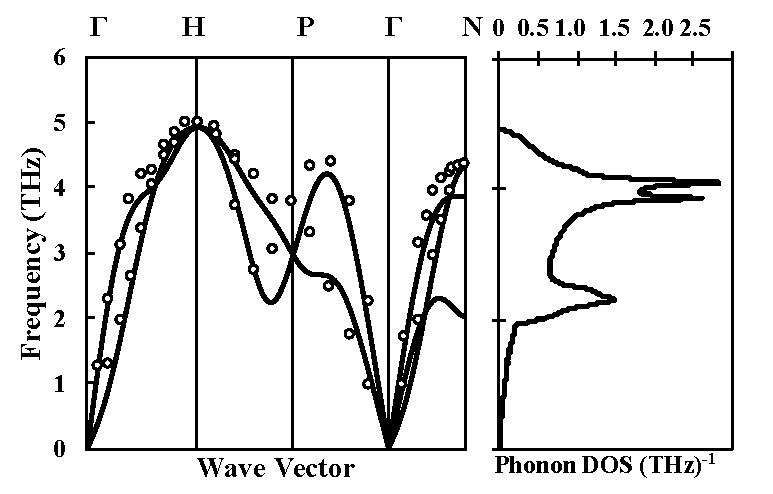
\includegraphics[width=\textwidth]{Chapter-4/Figures/Taphonondos.pdf}
	\caption{Calculated phonon dispersion curve of bcc-Ta, compared with neutron diffraction experiments ($\circ$) \cite{Taioli2007a} along with the phonon DOS. }
	\label{Ch4-figure:Taphonon}
\end{figure}

\pagebreak
\begin{figure}[H]
	\centering
	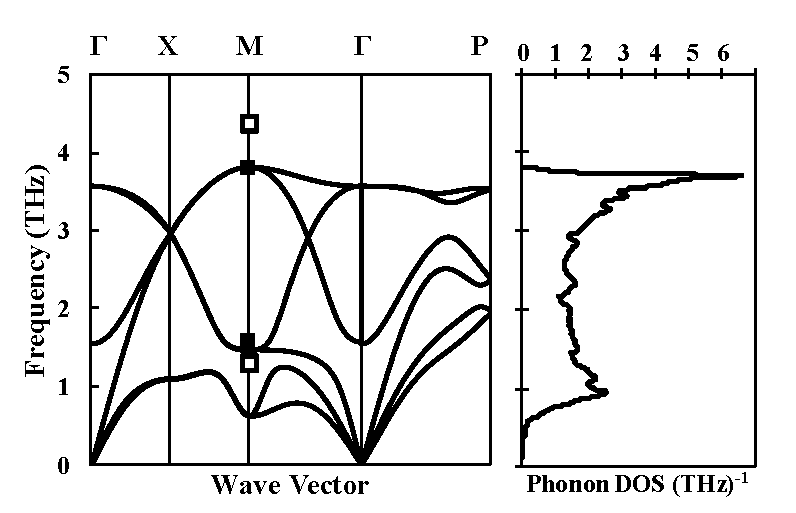
\includegraphics[width=\textwidth]{Chapter-4/Figures/Snphonondos.pdf}
	\caption{Calculated phonon dispersion curve of bct-Sn on the left and phonon DOS on the right. The open squares ($\square$) are the LO and TO modes from Raman \cite{Olijnyk1992} and the filled squares the theoretical prediction of the LO and TO modes at the M point \cite{Olijnyk1992}.}
	\label{Ch4-figure:Snphonon}
\end{figure}

\pagebreak
\begin{figure}[H]
	\centering
	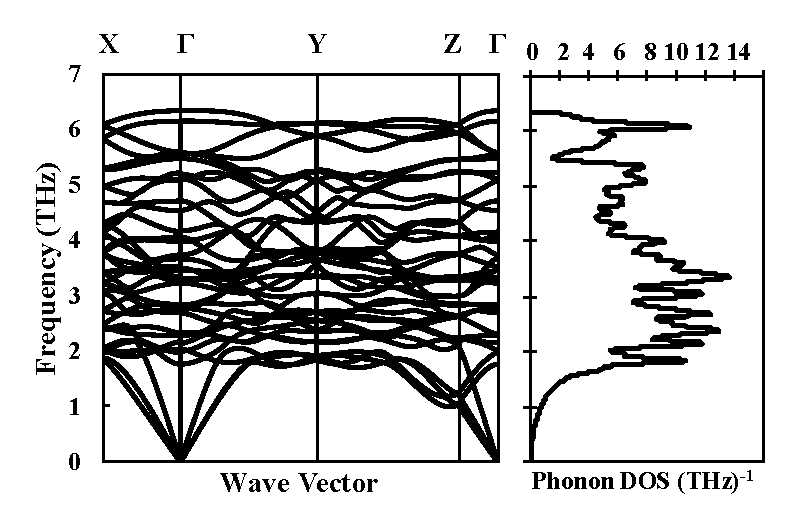
\includegraphics[width=\textwidth]{Chapter-4/Figures/TaSn2phonondos.pdf}
	\caption{Calculated phonon dispersion curve for TaSn$_2$ at 0 $^\circ$K and the phonon DOS.}
	\label{Ch4-figure:TaSn2phonon}
\end{figure}

\pagebreak
\begin{figure}[H]
	\centering
	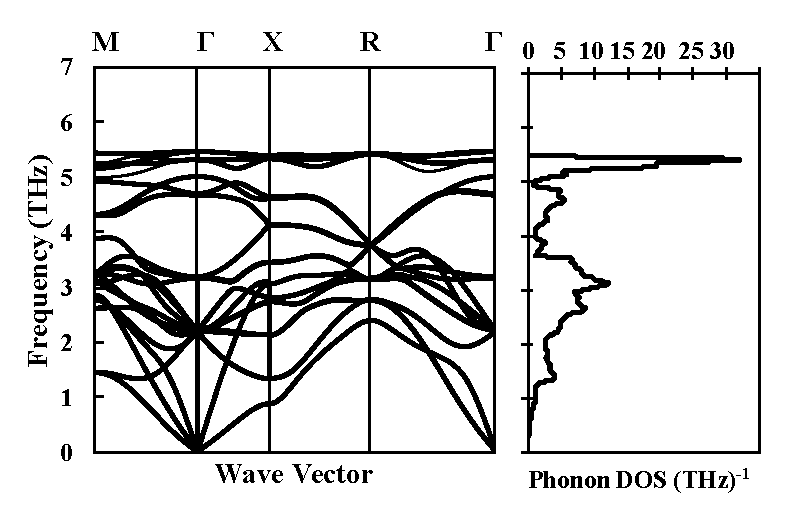
\includegraphics[width=\textwidth]{Chapter-4/Figures/Ta3Snphonondos.pdf}
	\caption{Calculated phonon dispersion curve of Ta$_3$Sn at 0 $^\circ$K on the left and the phonon DOS on the right.}
	\label{Ch4-figure:Ta3Snphonon}
\end{figure}

\pagebreak
\begin{figure}[H]
	\centering
	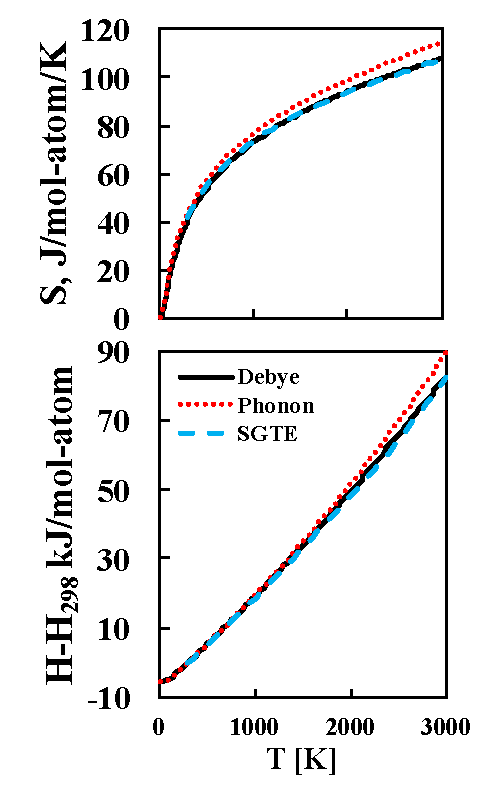
\includegraphics[scale=1.0]{Chapter-4/Figures/Tafinitetemp.pdf}
	\caption{Comparison of the enthalpy and entropy of bcc-Ta from the Debye model (solid line) and the quasiharmonic phonon calculations (red dotted line) to the SGTE data (blue dashed line) \cite{Dinsdale1991}.}
	\label{Ch4-figure:Tafinitetemp}
\end{figure}

\pagebreak
\begin{figure}[H]
	\centering
	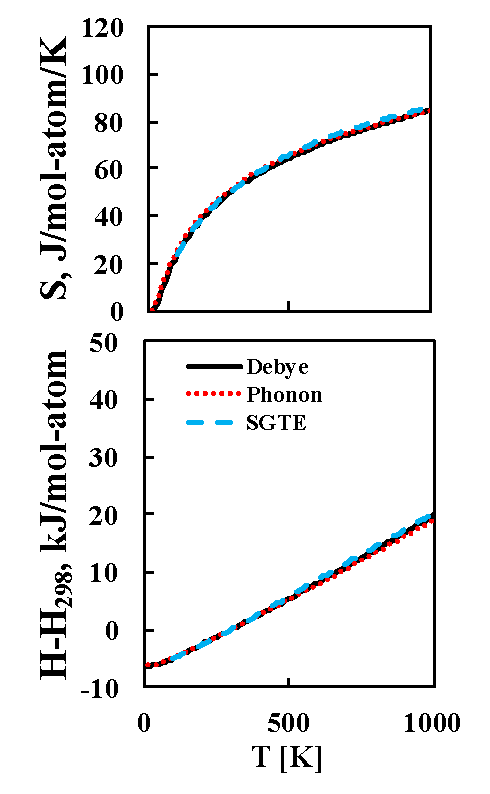
\includegraphics[scale=1.0]{Chapter-4/Figures/Snfinitetemp.pdf}
	\caption{Comparison of the Gibbs energy of bct-Sn from the Debye model (solid line) and the quasiharmonic phonon calculations (red dotted line) to the SGTE data (blue dashed line) \cite{Dinsdale1991}.}
	\label{Ch4-figure:Snfinitetemp}
\end{figure}

\pagebreak
\begin{figure}[H]
	\centering
	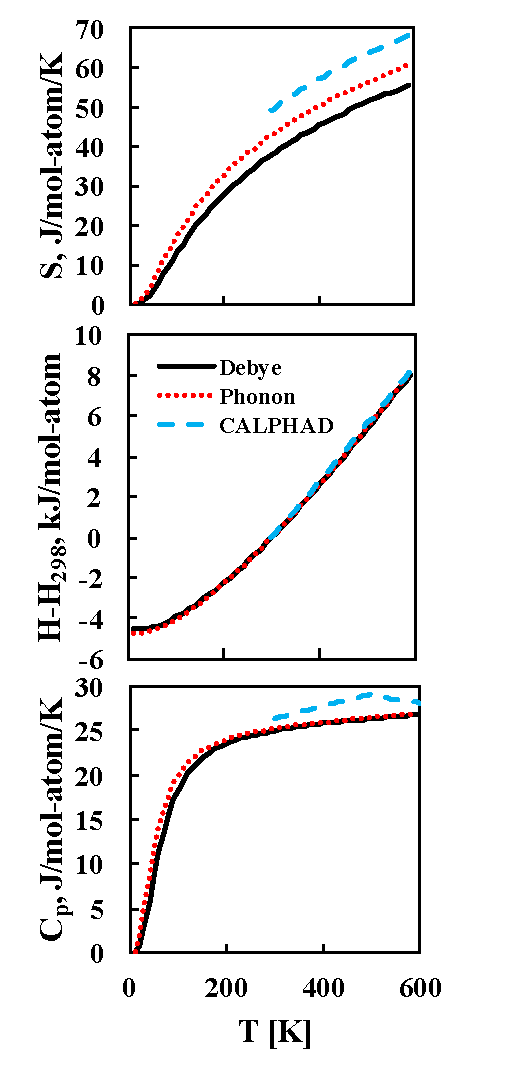
\includegraphics[scale=1.0]{Chapter-4/Figures/TaSn2finitetemp.pdf}
	\caption{Heat capacity, enthalpy and entropy of TaSn$_2$ using the Debye model (solid line) and the quasiharmonic phonon calculation (red dotted line) from first-principles calculations, compared with those from the current CALPHAD modeling (blue dashed line).}
	\label{Ch4-figure:TaSn2finitetemp}
\end{figure}

\pagebreak
\begin{figure}[H]
	\centering
	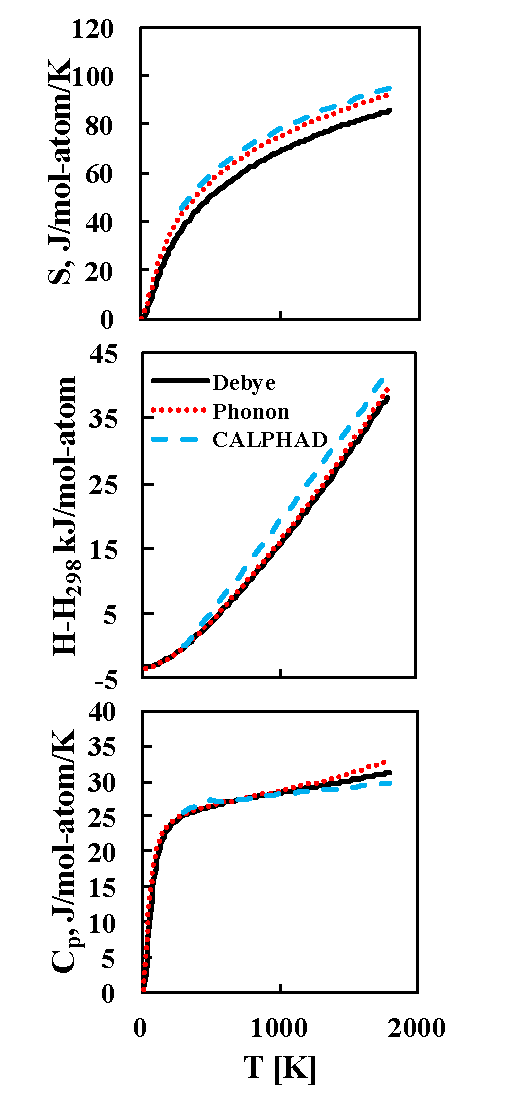
\includegraphics[scale=1.0]{Chapter-4/Figures/Ta3Snfinitetemp.pdf}
	\caption{Heat capacity, enthalpy and entropy of Ta$_3$Sn using the Debye model (solid line) and the quasiharmonic phonon calculation (red dotted line) compared with those from the current CALPHAD modeling (blue dashed line).}
	\label{Ch4-figure:Ta3Snfinitetemp}
\end{figure}

\pagebreak
\begin{figure}[H]
	\centering
	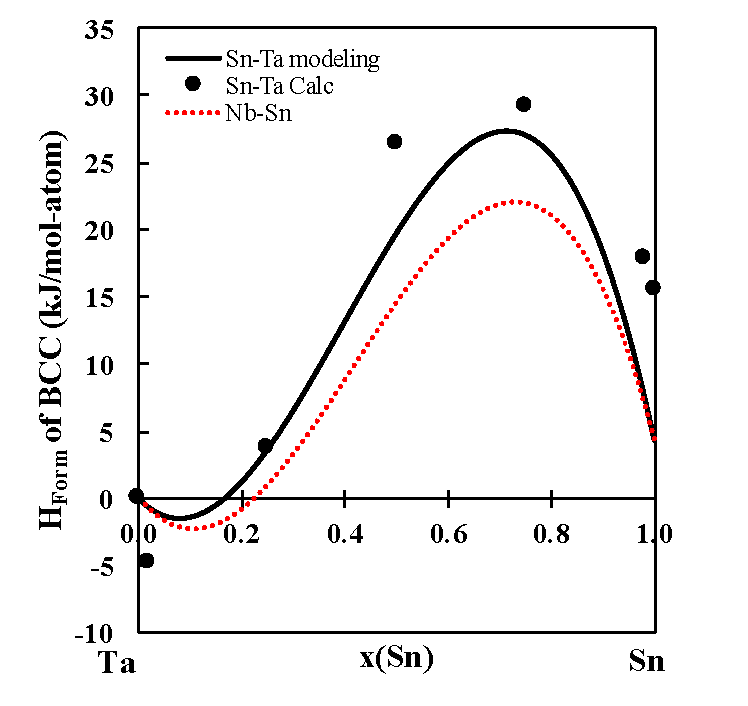
\includegraphics[width=\textwidth]{Chapter-4/Figures/HofForm.pdf}
	\caption{Enthalpy of formation of the bcc phase of the Sn-Ta system as a function of composition at 298 $^{\circ}$K and ambient pressure from the current CALPHAD modeling (solid line) and from the first-principles calculations (dots), showing asymmetric behavior. This was compared with data of the Nb-Sn system from Toffolon et al. \cite{Toffolon1998} (dashed red line) which was modeled using experimental data, showing similar asymmetric behavior.}
	\label{Ch4-figure:HofForm}
\end{figure}

\pagebreak
\begin{figure}[H]
	\centering
	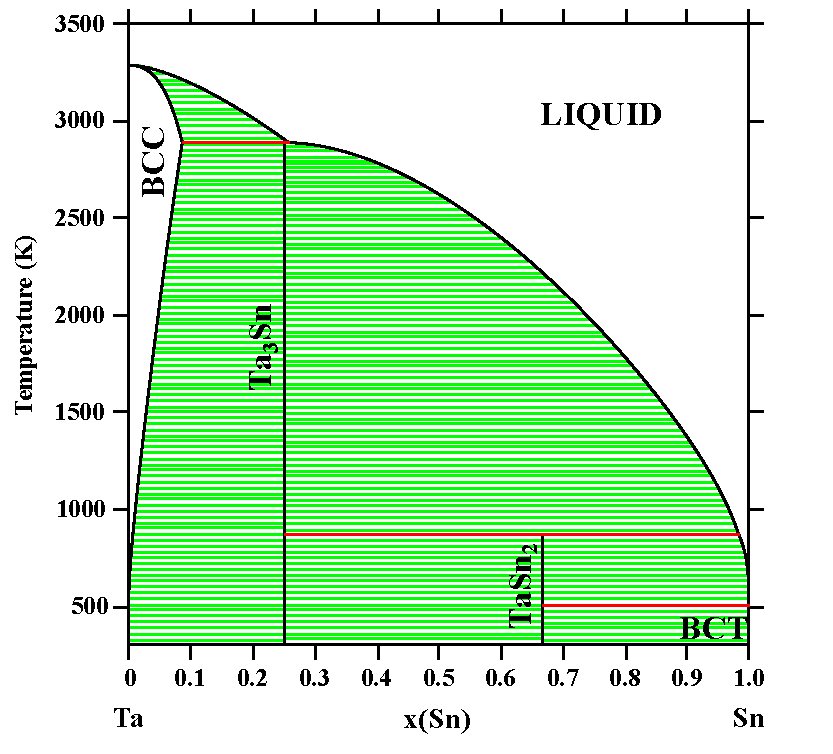
\includegraphics[width=\textwidth]{Chapter-4/Figures/SnTaPD.pdf}
	\caption{Calculated Sn-Ta phase diagram using the present thermodynamic description.}
	\label{Ch4-figure:SnTaPD}
\end{figure}

\pagebreak
\begin{figure}[H]
	\centering
	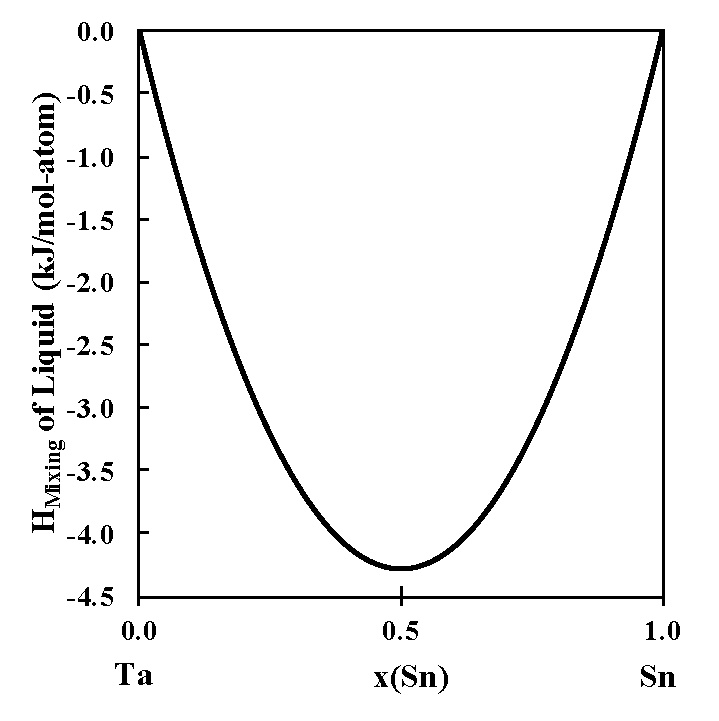
\includegraphics{Chapter-4/Figures/HofMix.pdf}
	\caption{Enthalpy of mixing of the liquid phase as a function of composition at 298 $^\circ$K and ambient pressure in the Sn-Ta system.}
	\label{Ch4-figure:HofMix}
\end{figure}